%


\documentclass[twoside]{article}
\setlength{\oddsidemargin}{0.25 in}
\setlength{\evensidemargin}{-0.25 in}
\setlength{\topmargin}{-0.6 in}
\setlength{\textwidth}{6.5 in}
\setlength{\textheight}{8.5 in}
\setlength{\headsep}{0.75 in}
\setlength{\parindent}{0 in}
\setlength{\parskip}{0.1 in}

%
% ADD PACKAGES here:
%

\usepackage{amsmath,amsfonts,graphicx}

%
\newcounter{lecnum}
\renewcommand{\thepage}{\thelecnum-\arabic{page}}
\renewcommand{\thesection}{\thelecnum.\arabic{section}}
\renewcommand{\theequation}{\thelecnum.\arabic{equation}}
\renewcommand{\thefigure}{\thelecnum.\arabic{figure}}
\renewcommand{\thetable}{\thelecnum.\arabic{table}}

%
% The following macro is used to generate the header.
%
\newcommand{\lecture}[4]{
   \pagestyle{myheadings}
   \thispagestyle{plain}
   \newpage
   \setcounter{lecnum}{#1}
   \setcounter{page}{1}
   \noindent
   \begin{center}
   \framebox{
      \vbox{\vspace{2mm}
    \hbox to 6.28in { {\bf EE402 - Discrete Time Systems
	\hfill Spring 2018} }
       \vspace{4mm}
       \hbox to 6.28in { {\Large \hfill Lecture #1 \hfill} }
       \vspace{2mm}
       \hbox to 6.28in { {\it Lecturer: #2 \hfill } }
      \vspace{2mm}}
   }
   \end{center}
   \markboth{Lecture #1}{Lecture #1}

   \vspace*{4mm}
}
%
% Convention for citations is authors' initials followed by the year.
% For example, to cite a paper by Leighton and Maggs you would type
% \cite{LM89}, and to cite a paper by Strassen you would type \cite{S69}.
% (To avoid bibliography problems, for now we redefine the \cite command.)
% Also commands that create a suitable format for the reference list.
\renewcommand{\cite}[1]{[#1]}
\def\beginrefs{\begin{list}%
        {[\arabic{equation}]}{\usecounter{equation}
         \setlength{\leftmargin}{2.0truecm}\setlength{\labelsep}{0.4truecm}%
         \setlength{\labelwidth}{1.6truecm}}}
\def\endrefs{\end{list}}
\def\bibentry#1{\item[\hbox{[#1]}]}

%Use this command for a figure; it puts a figure in wherever you want it.
%usage: \fig{NUMBER}{SPACE-IN-INCHES}{CAPTION}
\newcommand{\fig}[3]{
			\vspace{#2}
			\begin{center}
			Figure \thelecnum.#1:~#3
			\end{center}
	}
% Use these for theorems, lemmas, proofs, etc.
\newtheorem{theorem}{Theorem}[lecnum]
\newtheorem{lemma}[theorem]{Lemma}
\newtheorem{proposition}[theorem]{Proposition}
\newtheorem{claim}[theorem]{Claim}
\newtheorem{corollary}[theorem]{Corollary}
\newtheorem{definition}[theorem]{Definition}
\newenvironment{proof}{{\bf Proof:}}{\hfill\rule{2mm}{2mm}}

% **** IF YOU WANT TO DEFINE ADDITIONAL MACROS FOR YOURSELF, PUT THEM HERE:

\begin{document}

% Lecture Details
\lecture{11}{Asst. Prof. M. Mert Ankarali}
....

\section*{Frequency Response in Discrete Time Control Systems}

Let's assume $u[k]$, $y[k]$, and $G(z)$ represents the input, output,
and transfer function representation of an input-output discrete time
system.

In order to characterize frequency response of a discret system,
the test signal is 
%
\begin{align*}
 u[k] = e^{j \omega k}
\end{align*}
%
which is an artificial complex periodic signal with a DT domain
frequency of $\omega$. The z-transform of $u[k]$ takes the
form
%
%
\begin{align*}
 U(z) = \mathcal{Z} \lbrace e^{j \omega k} \rbrace = \frac{z}{z - e^{j \omega}}
\end{align*}
%
Response of the system in z-domain is given by
%
%
\begin{align*}
 Y(z) = G(z) U(z) = G(z) \frac{z}{z - e^{j \omega}}
\end{align*}
%
Assuming that $G(z)$ is a rational transfer function
we can perform a partial fraction expansion
%
\begin{align*}
     Y(z) &= \frac{a z}{z -  e^{j \omega}} + \left[ \mathrm{terms \ due \
  to \ the \ poles \ of} \  G(z) \right] 
\\
a &= \lim_{z \to e^{j \omega}} \left[ (z - e^{j \omega}) \frac{Y(z)}{z}
  \right]  = G(e^{j \omega})
\\
Y(z) &=  \frac{G(e^{j \omega}) z}{z -  e^{j \omega}} + \left[ \mathrm{terms \ due \
  to \ the \ poles \ of} \  G(z) \right]  
\end{align*}
%
Taking the inverse z-transform yields
%
\begin{align*}
  y(t) = G(e^{j \omega}) e^{j \omega k} + \mathcal{Z}^{-1} \left[ \mathrm{terms \ due \
  to \ the \ poles \ of} \  G(z) \right]  
\end{align*}
%
If we assume that the system is ``stable'' or system is a part of
closed loop system and closed loop behavior is stable then
at steady state we have
%
\begin{align*}
y_{ss}[k] &= G(e^{j \omega}) e^{j \omega k} \\
&= | G(e^{j \omega}) | e^{i \omega k + \angle G(e^{j \omega})}
\\
&= M e^{i \omega k + \theta}
\end{align*}
%
In other words complex periodic signal is scaled and phase shifted
based on the following operators
%
\begin{align*}
M &= | G(e^{j \omega}) | \\
\theta &= \angle G(e^{j \omega})
\end{align*}
%
It is very easy to show that for a general real time domain signal
$u[k] = \sin (\omega k + \phi)$, the output $y[k]$ at steady state 
is computed via
%
\begin{align*}
  y_{ss}[k] = M \sin(\omega k + \phi + \theta)
\end{align*}
%
If there is sampling involved in the system the following relation
between DT frequency and CT frequency exists $\omega_d = \omega_c T$

Similar to CT systems we utilize bode polts (or FRF function polts) to
analyze DT systems and design filters/controllers. Main difference
between CT and DT bode polt is that while the frequency goes to
infinity for CT bode polts, for DT systems the frequency goes up-to
$\pi \ \mathrm{rad}$ or  $\omega_s / 2$ (i.e. Nyquist frequency). 
Given the bode polt one can extract the magnitude scale and phase 
difference with respect to any input frequency. 

\textbf{Example:} Let's assume that we have the following 
CT plant transfer function
%
\begin{align*}
  G(s) = \frac{1}{s+1}
\end{align*}
%
The pulse transfer function of the following discretized 
system can be computed as
%
%
\begin{align*}
  G(z) = \mathcal{Z} \left[ \frac{1-e^{-Ts}}{s} \frac{1}{s+1} \right] 
\end{align*}
%
     \begin{center}
 \begin{minipage}[h]{\linewidth}
     \begin{center}
       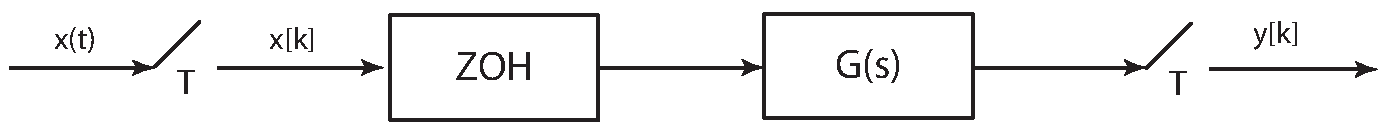
\includegraphics[width=\textwidth]{Gz}
     \end{center}
 \end{minipage}
     \end{center}
%
We can also transform this DT transfer function to an 
artificial CT form using Bilinear-Tustin transformation.
%
%
\begin{align*}
  G(\bar{s}) = G(z) |_{z = \frac{1 + (T/2) \bar{s}}{1 - (T/2) \bar{s}}} 
\end{align*}
%
Now let's draw the bode plots of $G(s)$, $G(z)$, and $G(\bar{s})$
for both $T = 0.01 s$ and $T = 0.001 s$.

\begin{center}
 \begin{minipage}[h]{0.99\linewidth}
     \begin{center}
       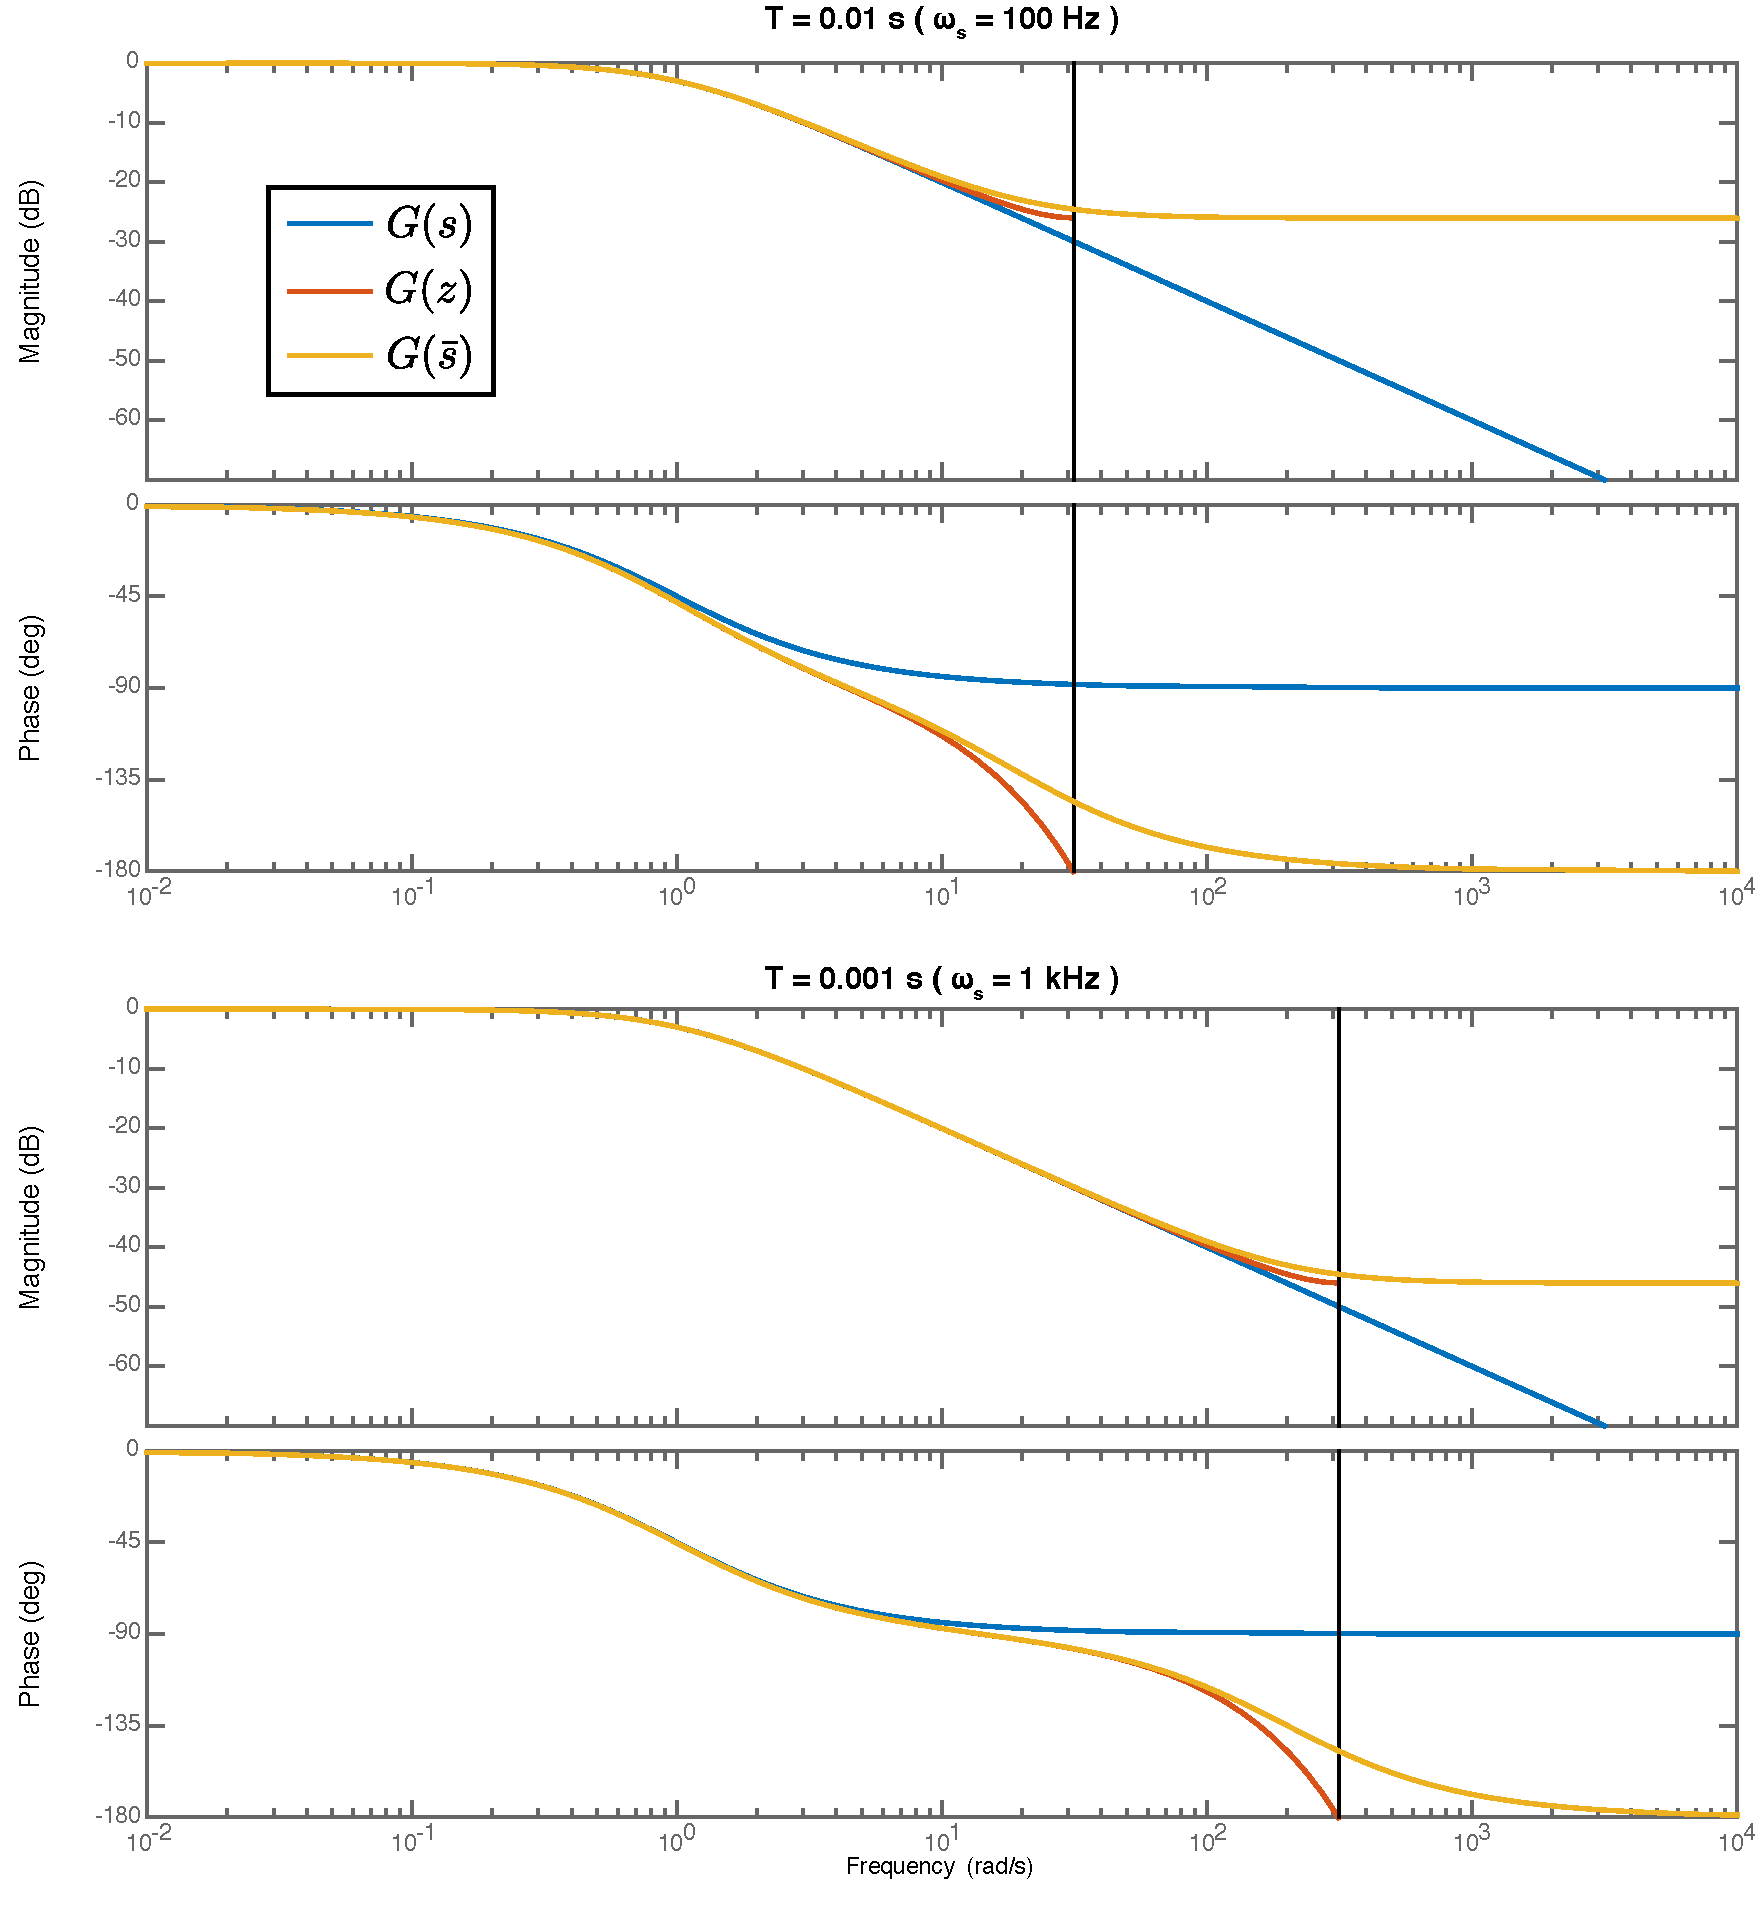
\includegraphics[width=\textwidth]{bode_all}
     \end{center}
 \end{minipage}
\end{center}

\newpage

\section*{Phase and Gain Margins}

We already know that a binary stability metric is not enough to
characterize the system performance and that we need metrics
to evaluate how stable the system is and its robustness to
perturbations. Using root-locus techniques we talked about
some ``good'' pole regions which provides some specifications
about stability and closed-loop performance. 

Another common and powerful method is to use gain and phase margins
based on the Frequency Response Functions of a closed-loop topology. 
Phase and gain margins are derived from the Nyquist’s stability
criterion and it is relatively easy to compute them from the Bode diagrams.

\subsection*{Gain Margin}

The \textit{gain margin}, $g_m$, of a system is defined as the smallest amount
that the open loop gain can be increased before the closed loop system 
goes unstable. For a system, whose ``open-loop'' phase response starts from an angle
$> -180^o$ at $\omega = 0$, the gain margin can be computed based on 
the smallest frequency where the phase of the loop transfer function
$G_{OL}(s)$ is $-180^o$. Let $\omega_{pc}$ represent this frequency,
called the phase crossover frequency. Then the gain margin for the
system is given by

\begin{align*}
  g_m = \frac{1}{| G_{OL}(j \omega_{pc})| } \quad \mathrm{or} \quad G_m
  = -20 \,
  \mathrm{log}_{10} | G_{OL}(j \omega_{pc} ) |
\end{align*}

where $G_m$ is the gain margin in dB scale. 

If the phase response never crosses the $-180^o$ line, gain margin is simply $\infty$.

\subsection*{Phase Margin}

The \textit{phase margin} is the amount of ``phase lag'' required to
reach the (Nyquist) stability limit. Let $\omega_{gc}$ be the gain
crossover frequency, the smallest frequency where the loop transfer 
function $G_{OL}(s)$ has unit magnitude. Then for a system for which
the gain response at $\omega = 0$ is larger than $1$ and gain
decreases and eventually crosses the unity gain line, the phase margin 
is given by

\begin{align*}
  \phi_m = \pi + \angle G_{OL} (j \omega_{gc})
\end{align*}

When the gain and phase plots shows monotonic like 
behaviors gain and phase margins becomes more 
meaningful in terms of closed-loop performance.

So far we have only talked about stability margins for a
CT control system. Indeed, the Nyquist stability criterion 
and associated phase and gain margin definitions
are almost exactly same, if we consider FRF functions.
Let $G_{OL}(z)$ be the open-loop pulse transfer function
of a discrete time control system, then the gain and
phase margins are computed as

\begin{align*}
    g_m &= \frac{1}{| G_{OL}(e^{j \omega_{wc})} |} \quad \mathrm{or} \quad G_m
  = -20 \,
  \mathrm{log}_{10} | G_{OL}(e^{j \omega_{wc} }) |
\\
  \phi_m &= \pi + \angle G_{OL} (e^{j \omega_{gc}})
\end{align*}

where as definitions of gain and phase crossover frequencies are 
exactly same.

\textbf{Example:} Let's consider a CT plant transfer function
%
\begin{align*}
  G(s) = \frac{3}{(s+1)^3}
\end{align*}
%
Nyquist plot, bode diagrams are illustrated in the given Figure below
%
\begin{center}
\begin{minipage}[h]{\linewidth}
    \begin{center}
      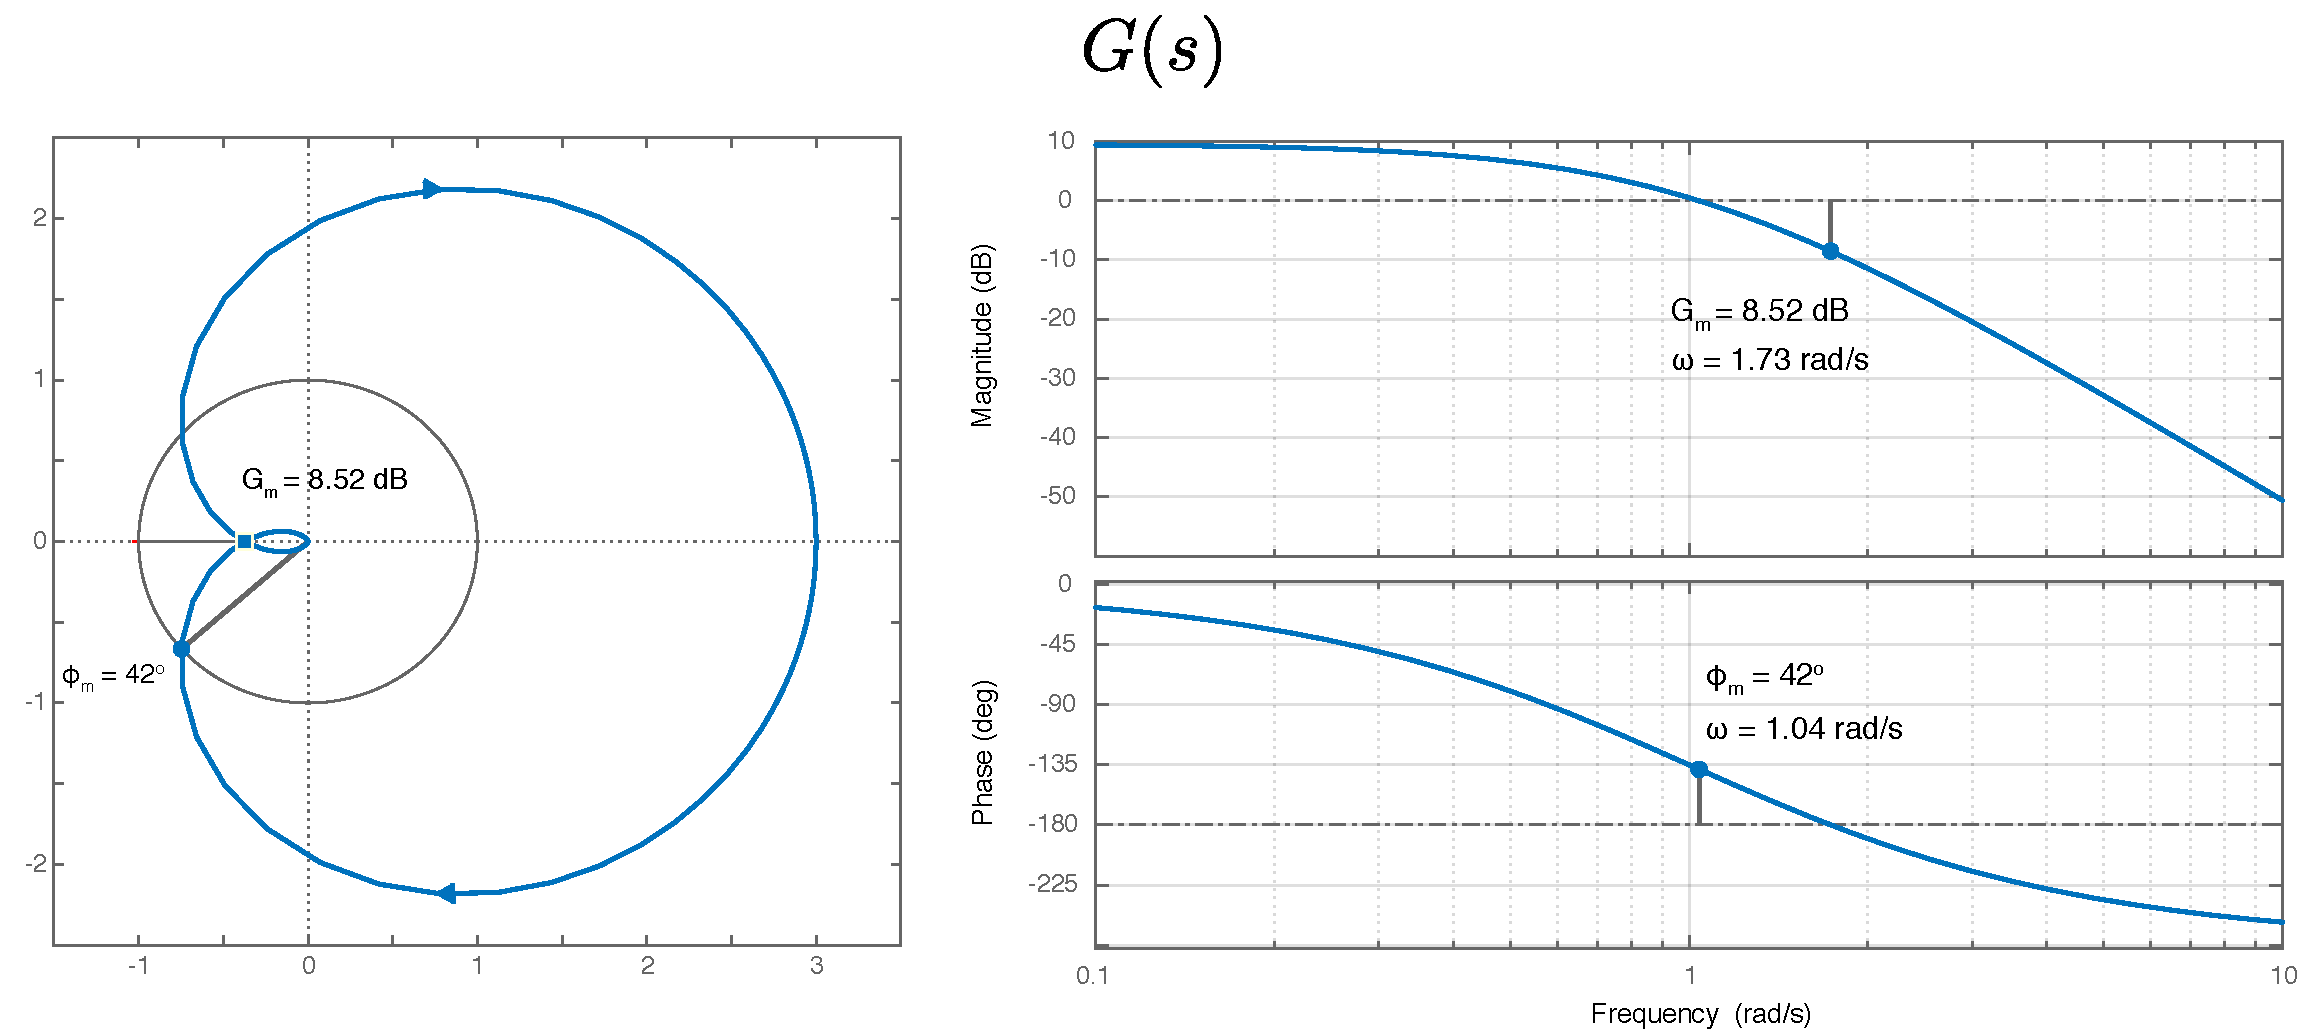
\includegraphics[width=\textwidth]{Gp}
    \end{center}
\end{minipage}
\end{center}
%
The phase crosover frequency and gain margin for the CT open-loop
transfer function is given below
%
\begin{align*}
\omega_{pc} &= 1.73 \ \mathrm{rad/s} 
\\
g_m &= \frac{1}{| G(j \omega_{pc}|} = 2.67 
\\
G_m &= 8.5 dB
\end{align*}
%
On the other hand gain crosover frequency and phase margin 
for $G(s)$ is computed as
%
\begin{align*}
\omega_{gc} &= 1.04 \ \mathrm{rad/s} 
\\
\phi_m &= \pi + \angle G(j \omega_{pc}) = 42^0
\end{align*}
%
Now let's assume that this plant transfer function
is controlled via a unity gain digital feedback 
controller and a ZOH operator, where sampling time
is $T = 0.5 \ s$. Open-loop pulse transfer function
can be found as
%
\begin{align*}
  G(z) = \left[ \frac{1 - e^{-Ts}}{s} G(s) \right] 
\end{align*}
%
The Nyquist and bode polts for this DT open-loop
puls transfer function is illustrated below
%
\begin{center}
\begin{minipage}[h]{\linewidth}
    \begin{center}
      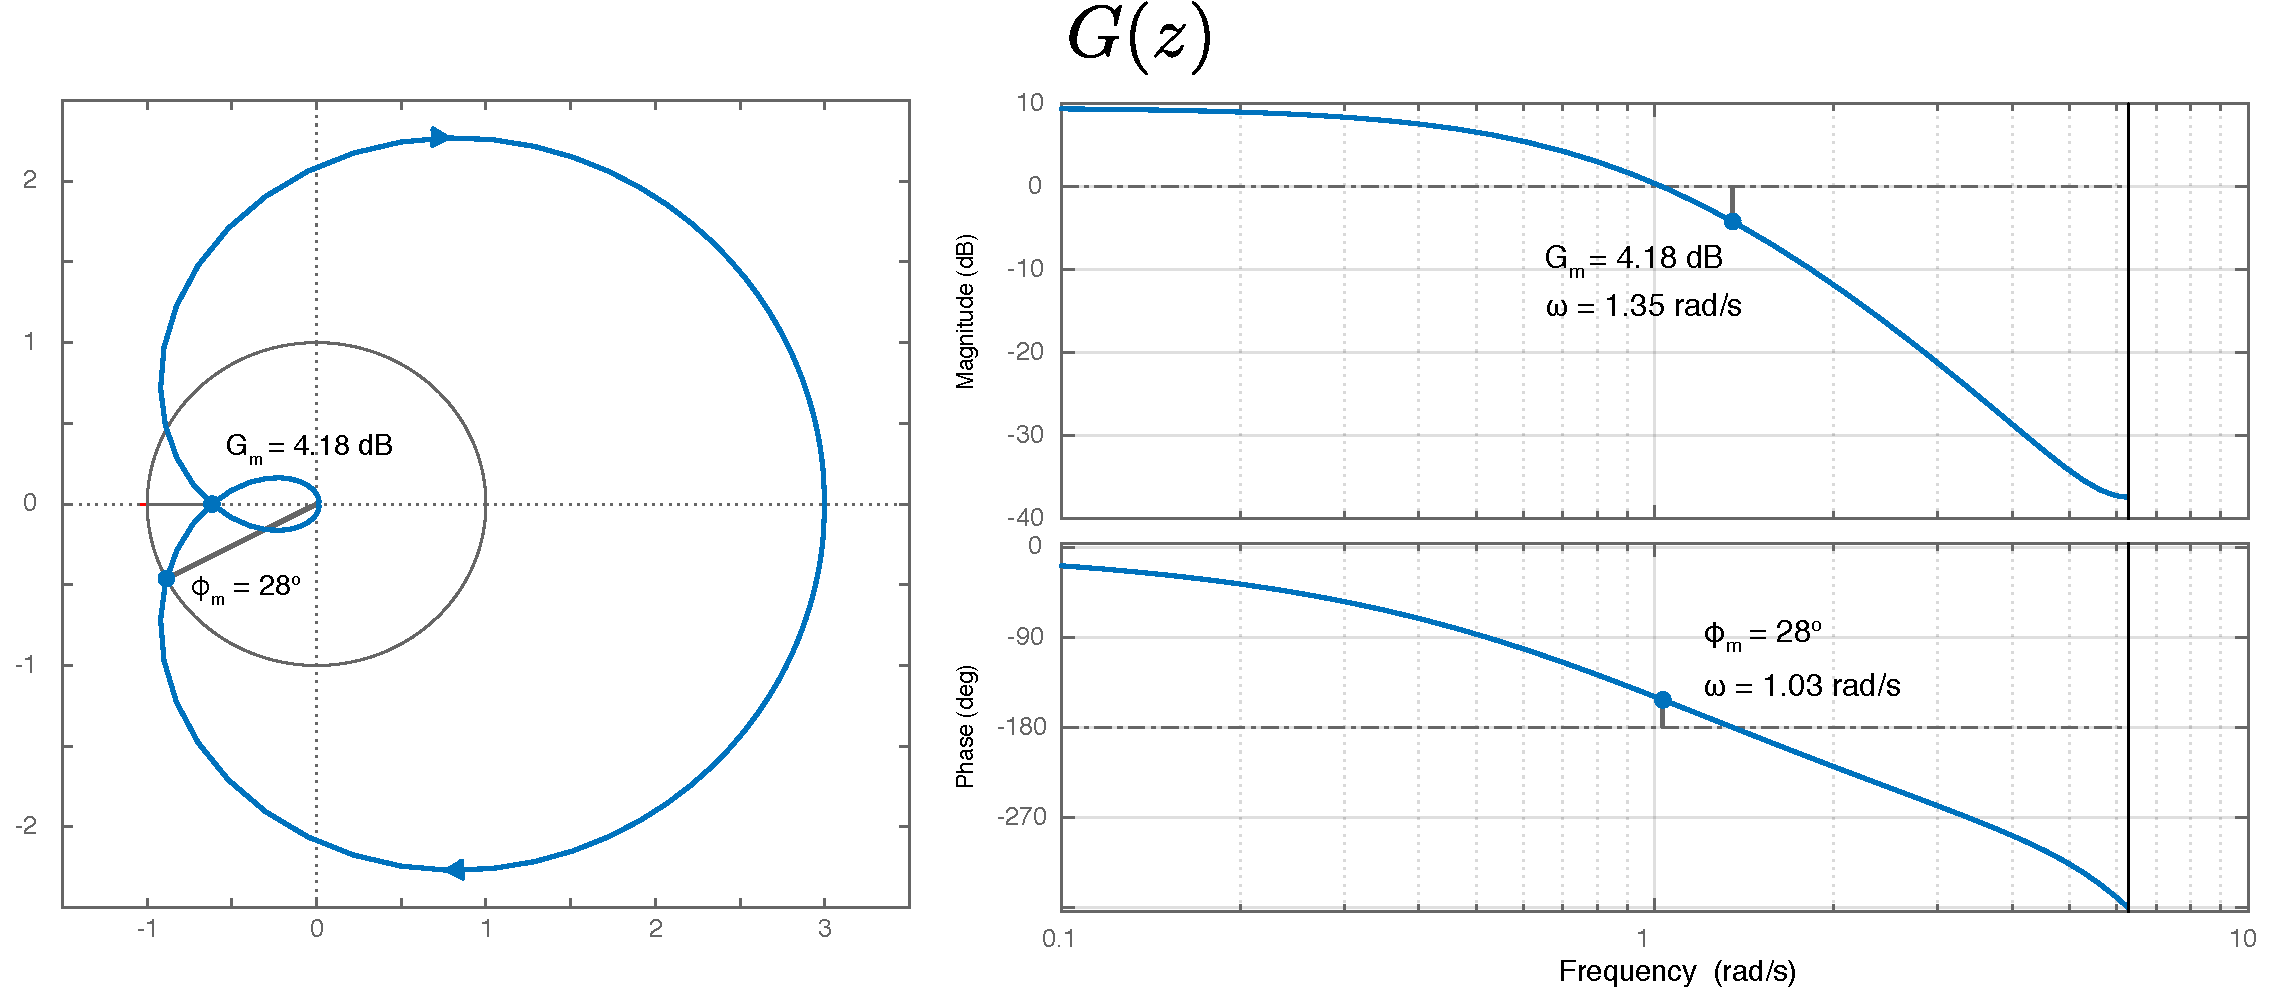
\includegraphics[width=\textwidth]{Gd}
    \end{center}
\end{minipage}
\end{center}
%
Note that instead of DT frequency $\omega_d \in [0, pi)$,
the x-axis illustrates the actual frequency $\omega = \omega_d / T $.
It is very easy to associate DT and CT frequencies, and main advantage 
of actual frequency is that CT and DT versions of bode plots
becomes directly comparable.

The phase crosover frequency and gain margin for the DT open-loop
transfer function is given below
%
\begin{align*}
\omega_{pc} &= 1.35 \ \mathrm{rad/s} 
\\
g_m &= \frac{1}{| G(e^{j \omega_{pc} T|}} = 1.62
\\
G_m &= 4.18 dB
\end{align*}
%
On the other hand gain crosover frequency and phase margin 
for $G(s)$ is computed as
%
\begin{align*}
\omega_{gc} &= 1.03 \ \mathrm{rad/s} 
\\
\phi_m &= \pi + \angle G(j \omega_{pc}| = 28^0
\end{align*}

If we compare the CT and DT versions of the same system, we can see 
that both gain margin and phase margin of the original CT system is
better, and we can conclude that discretization reduces the
``stability''. Another interesting result is that while there is a
significant change in phase-crossover frequency, the change in gain
crosover frequency is minimal. 

Now let's transfrom the $G(z)$ to a artificial CT system using 
Bilinear-Tustin transformation:
%
%
\begin{align*}
  G(\bar{s}) = G(z) |_{z = \frac{1 + (T/2) \bar{s}}{1 - (T/2) \bar{s}}}
\end{align*}
%
We know that the relation between the frequency of this 
artificial system, $\bar{\omega}$, and frequencies of the actual system
and discretized system are given by
%
\begin{align*}
\bar{\omega} = \frac{2}{T} \tan (\frac{\omega_d}{2}) = \frac{2}{T}
  \tan (\frac{\omega T}{2}) 
\end{align*}
%
%
\begin{center}
\begin{minipage}[h]{\linewidth}
    \begin{center}
      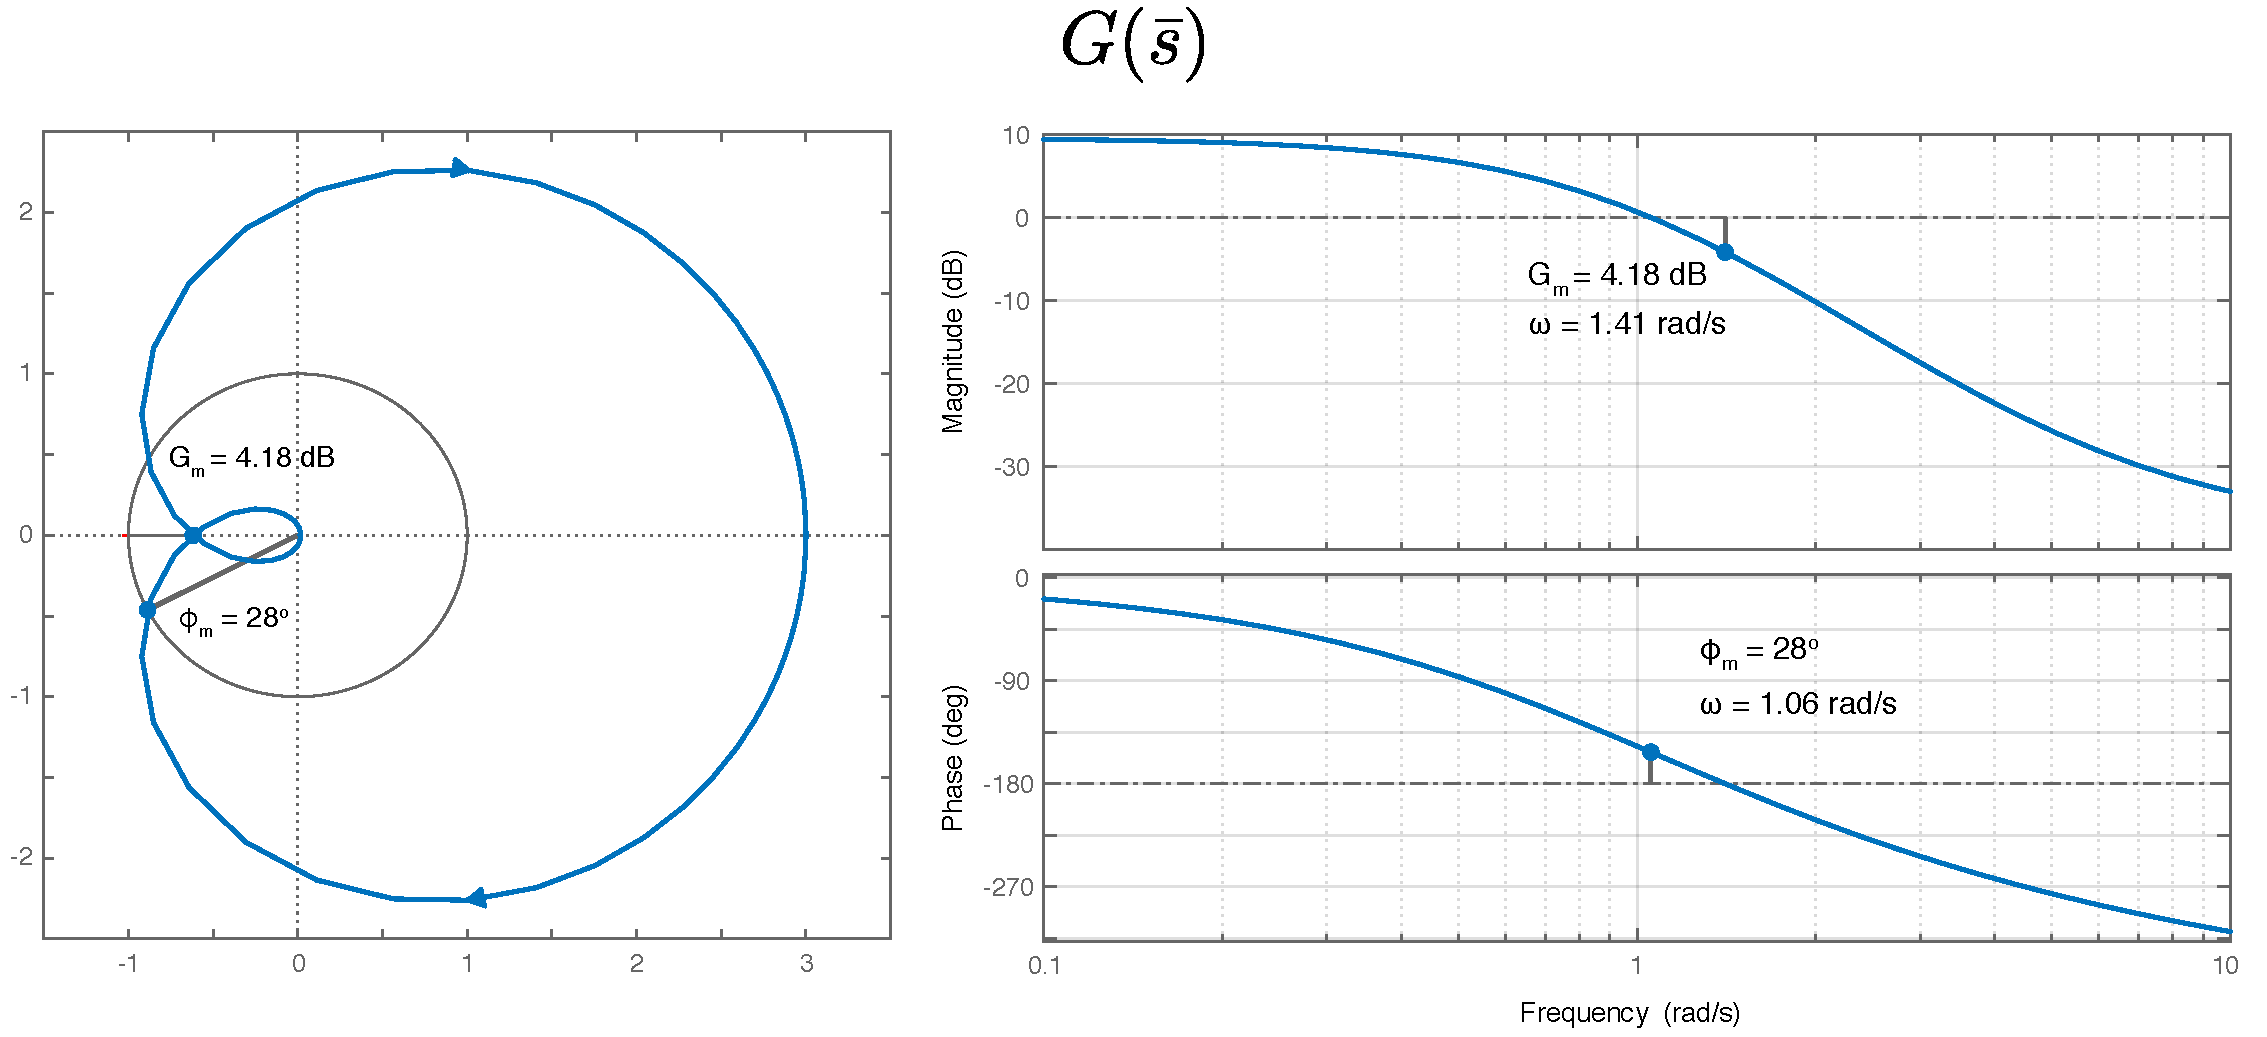
\includegraphics[width=\textwidth]{Gt}
    \end{center}
\end{minipage}
\end{center}
%

The phase crosover frequency and gain margin for this artificial CT open-loop
transfer function is given below
%
\begin{align*}
\omega_{pc} &= 1.41 \mathrm{rad/s} 
\\
g_m &= \frac{1}{| G(e^{j \omega_{pc} T|}} = 1.62
\\
G_m &= 4.18 dB
\end{align*}
%
On the other hand gain crosover frequency and phase margin 
for $G(s)$ is computed as
%
\begin{align*}
\omega_{gc} &= 1.06 \ \mathrm{rad/s} 
\\
\phi_m &= \pi + \angle G(j \omega_{pc}| = 28^0
\end{align*}

If we compare the phase and gain margin and associated
crosover frequencies we can see that stability margins of
DT and Tustin-Transformed are almost same. It is an expected
result, because the core purpose of Tustin transformation
is transforming a DT system to a CT form by preserving the
stability and other importan characteristics.

Tustin transformation has two basic advantages
%
\begin{itemize}
  \item It ``preserves'' the stability and robustness 
   characteristics of the digital control system.
  \item Even though bode polts of DT systems 
   are perfectly valid (and useful), due to periodicity in
   $\omega_d$ the some of the simplicities and
   advantages of CT bode plots are lost. Since Tustin
   transformed system is a CT representation, we
   still can use these simplicities and other advantages.
\end{itemize}

There two basic disadvantages of Tustin transformation
\begin{itemize}
  \item It has significant computational costs. However in 
   a computer environment these costs can be negligible.
  \item If one designs a controller in Tustin form, and then
  back-transformes the controller in DT form. For some class
  of controller the quantization effects can become important
   and deadly. 
\end{itemize}

\newpage

\textbf{Lead-Compensator Design for DT Control Systems}

Let's consider the DT control system below. Let's assume 
that $T = 0.1 s$
%
     \begin{center}
 \begin{minipage}[h]{\linewidth}
     \begin{center}
       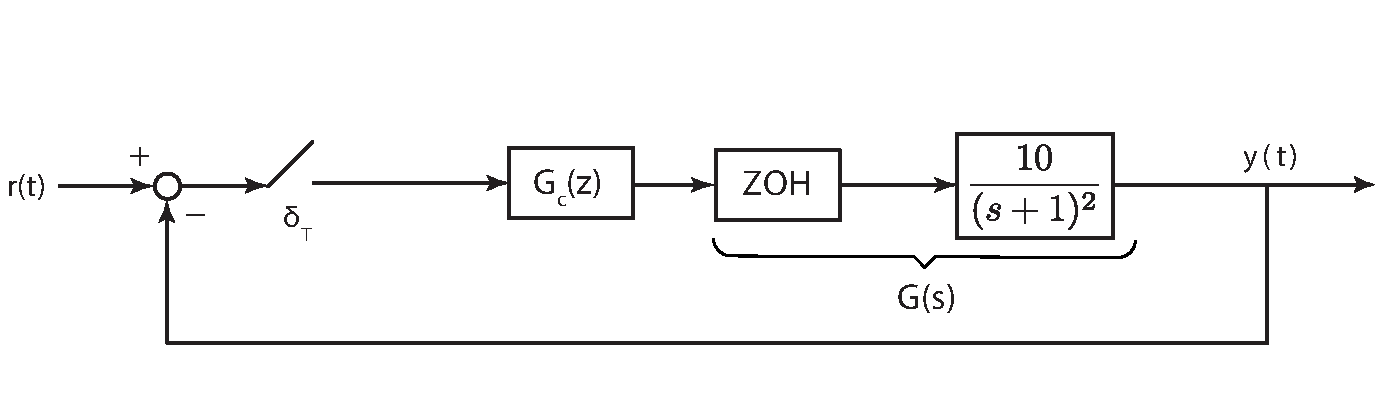
\includegraphics[width=\textwidth]{mainblock}
     \end{center}
 \end{minipage}
     \end{center}
%
The goal is designing a DT phase-lead compensator such that
the Phase-Margin is of the controlled system is in the desired 
range of $\phi_m \in [50^o \, 60^o]$.

Due to nice properties of CT bode plots, lead-compensator design 
procedure is handled in the Bilinear-Tustin transformed domain.
Below we will summarize the process for the example plant.

\begin{enumerate}
  \item Compute discretized plant transfer function $G(z)$
%
\begin{align*}
  G(z) &= \mathcal{Z} \left[ \frac{1-e^{-Ts}}{s} G_P(s) \right] 
\\
       &= \mathcal{Z} \left[ \frac{1-e^{-Ts}}{s} \frac{10}{(s+1)^2}
         \right] 
\\
&= \frac{0.047 z + 0.044}{z^2 - 1.8 z + 0.82}
\end{align*}
%
\item Compute the Bilinear-Tustin transformation of $G(z)$
%
\begin{align*}
  G(\bar{s}) &= G(z) |_{z = \frac{1 + (T/2) \bar{s}}{1 - (T/2)
  \bar{s}}} 
\\
&= \frac{ -0.0008 s^2 - 0.48 s + 9.98 }{s^2 + 2 s + 0.998}
\end{align*}
%

\item Now goal is designing a lead compensator for $G(\bar{s})$. 
Lead-compensator has the form.
%
\begin{align*}
  G_{l}(\bar{s}) = K_{\mathrm{lead}} \frac{T_{l} \ a \ s +
  1}{T_{l} /  a \ s + 1}
\end{align*}
%
where gain $K_{l}$ (generally) computed based on steady
state requirments. This can be computed either in z-domain or
s-bar domain. Let's assume that we are OK with steady-state 
performance and $K_{l} = 1$.

\item Compute the $\phi_m$ of the un-compensated system 
and find the required $\Delta \phi_m$ such that the 
compensated system meets the specifications.
%
\begin{align*}
  \phi_m &\approx 28^o
\\ 
  \Delta \phi_m &= [ 22^o \ , \ 32^o]
\end{align*}
%
     \begin{center}
 \begin{minipage}[h]{\linewidth}
     \begin{center}
       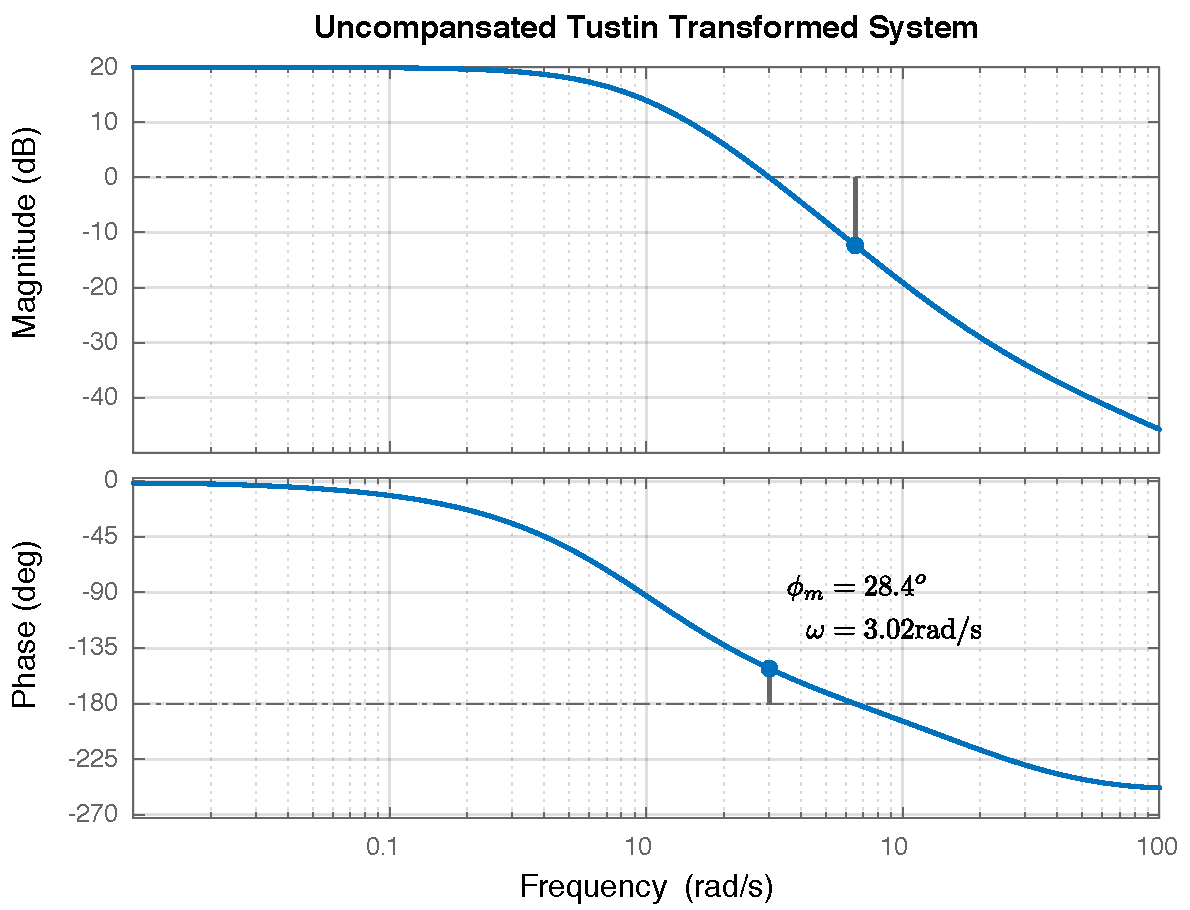
\includegraphics[width=\textwidth]{uncomp}
     \end{center}
 \end{minipage}
     \end{center}
%
\item For $a = 1.5$, $a = 2$, and $a = 3$, bode plots
of a phase-lead compensator is illustrated with $T_{l} = 1$
in the figure below.  
%
     \begin{center}
 \begin{minipage}[h]{\linewidth}
     \begin{center}
       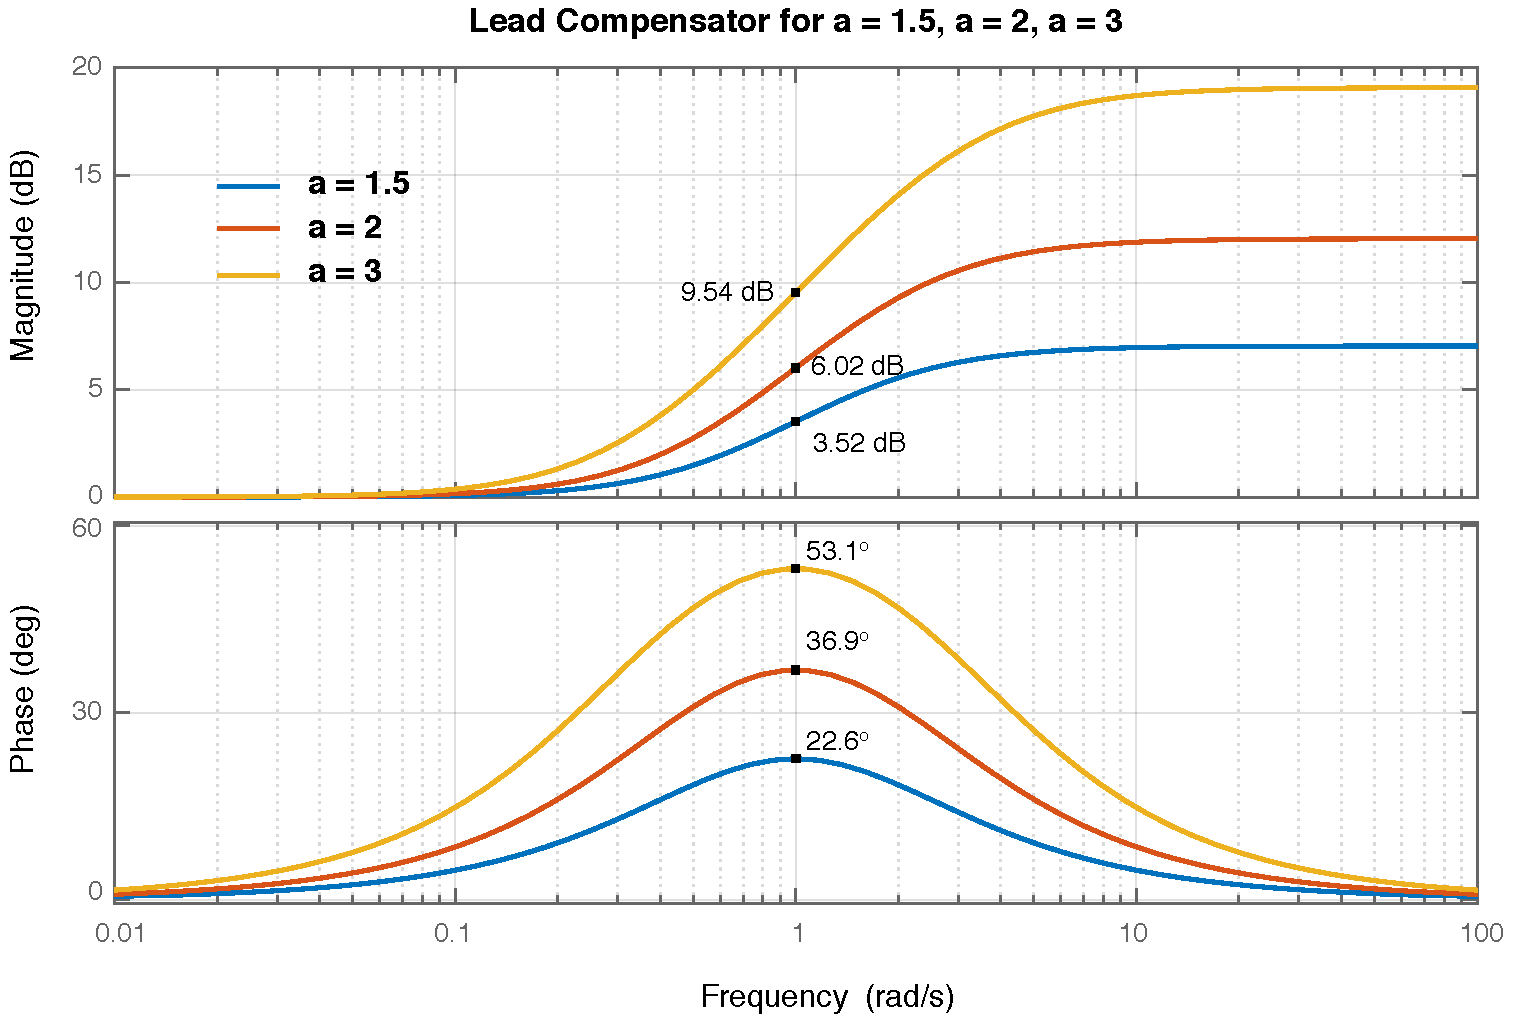
\includegraphics[width=\textwidth]{lead}
     \end{center}
 \end{minipage}
     \end{center}
%
It can be seen that $\phi_{max}$ is larger for large $a$.
$\phi_{max}$ (or $a$) can also be computed using the following
relation.
%
\begin{align*}
\sin \phi_{max} &=  \frac{a^2 - 1}{a^2 + 1}
\end{align*}
%
As your remember from EE302, Lead compensator should 
have a lead angle that is above $\approx 5-15^o$ the reqired
$\Delta \phi_m$. Based on this we compute/find $a$. 
Based on the bode polts, it seems that $a =2$
may supply the required additonal phase-margin.
One should see that $\phi_{max}$ is not affected
from the choice of $T_{l}$. 
%
\item Now our goal is to copmpute $T_{l}$, where $1/T_{l}$
corresponds to the center freqeuncy of the copmensator.
One possible choice is choosing $T$ such that 
$1/T_{l} = \bar{\omega}_{gc}$, i.e. gain croesover frequency.
However, at center frequency the lead copmensator
shifts the bode magnitude by
%
\begin{align*}
G_{\mathrm{center}} = 20 \mathrm{log}_{10} (1 / a)
\end{align*}
%
which causes a shift in gain-croesover frequency. 
For example, for $a = 2$, $G_{\mathrm{center}} \approx 6 \ dB$. 
For this reason, a ``better'' choice is choosing $T$ such that
center freqeuncy of the lead-compensator coincides with
the frequency where $|G(j \bar{\omega})|$ crosses 
$- 20 \ \mathrm{log}_{10} (1 / a)$, i.e. we compute $T_{l}$
such that
%
\begin{align*}
  |G(j 1/T_{l})| = - 20 \ \mathrm{log}_{10} (1 / a)
\end{align*}
%
From the bode polts for $a = 2$, the freqeuncy for which 
$G(\bar{s})$ croesses the $- 6 dB$ line is approximatelly 
$4.45 \ \mathrm{rad/s}$. Thus we choose $T = 0.225 s$.
Check if the lead-compensator meets the phase-margin
reqeuirment. Otherwise, repeat the process with a higher
$\delta \phi$ angle.

In our example, the resultant tustin domain lead compensator
has the form.
%
\begin{align*}
  G_{l}(\bar{s}) = \frac{0.45 s + 1}{0.1125 s + 1}
\end{align*}
%
The Figure below illiustrates the bode plots of both (tustin
domain) compensated and uncompansated systems.
Compensated systems has a phase margin of $\phi_m = 51^o$
which meets the requirements.
%
     \begin{center}
 \begin{minipage}[h]{\linewidth}
     \begin{center}
       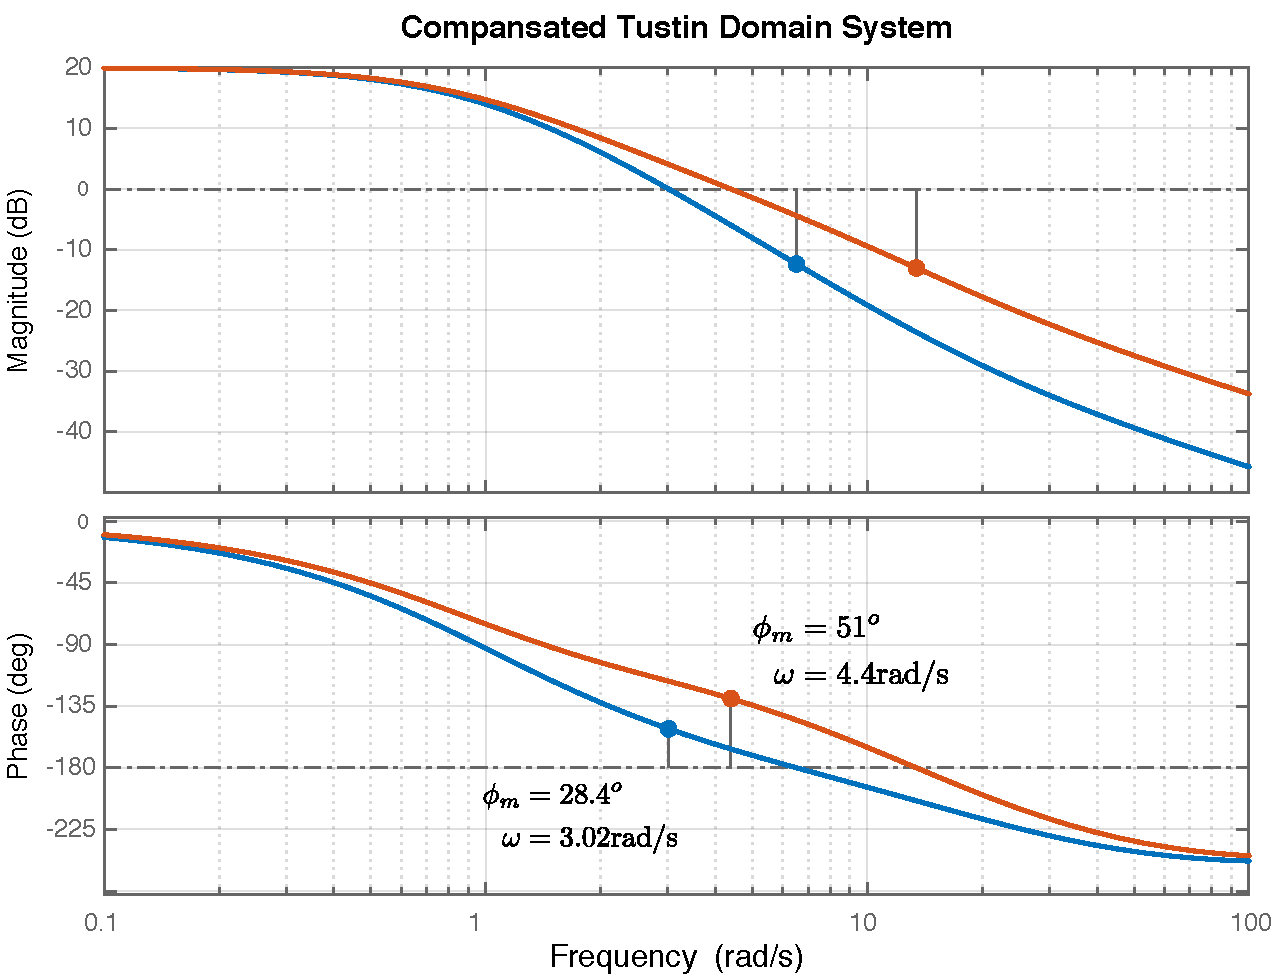
\includegraphics[width=\textwidth]{comptust}
     \end{center}
 \end{minipage}
     \end{center}
%
\item Transform the $\bar{s}$-domain lead-compensator
to z-domain.
%
\begin{align*}
  G_{l}(z) =& G_{l}(\bar{s})|_{\bar{s} = \frac{2}{T} \frac{z-1}{z+1}}
\\
  G_{l}(z) =& \frac{3.08 z - 2.46}{z - 0.385}
\end{align*}
%
\item Check if the discrete-time compensator meets the
the phse-margin requirments. 
%
     \begin{center}
 \begin{minipage}[h]{\linewidth}
     \begin{center}
       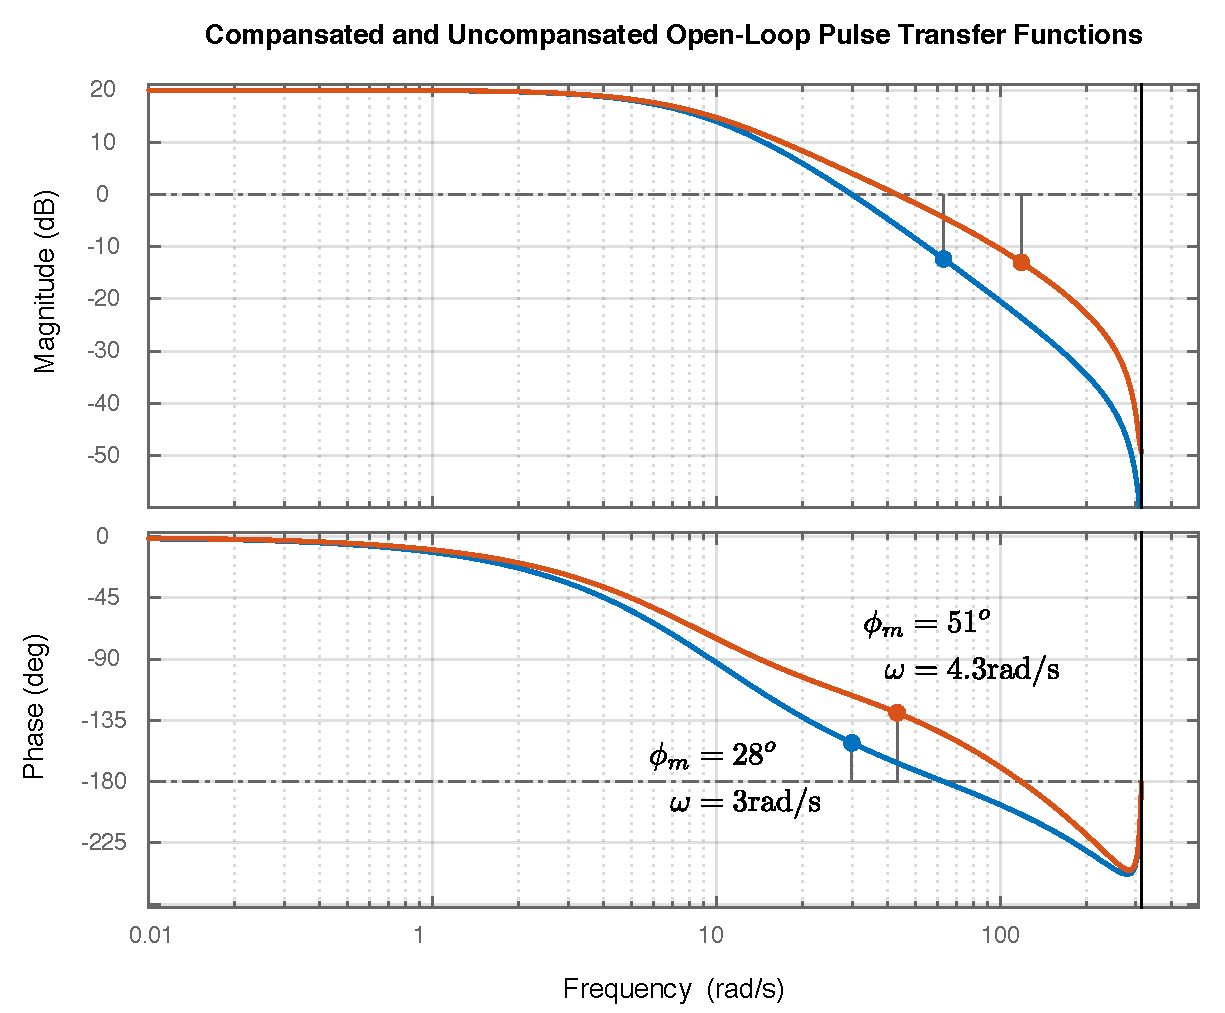
\includegraphics[width=\textwidth]{DTlead}
     \end{center}
 \end{minipage}
     \end{center}
%
It can be seen that the designed compensator in z-domain
also meets the phase-margin specifications.
%
\end{enumerate}

\newpage

In Figure below, we compare the closed-loop step responses
of both uncompensated and compensated pulse transfer functions.
%
     \begin{center}
 \begin{minipage}[h]{0.7\linewidth}
     \begin{center}
       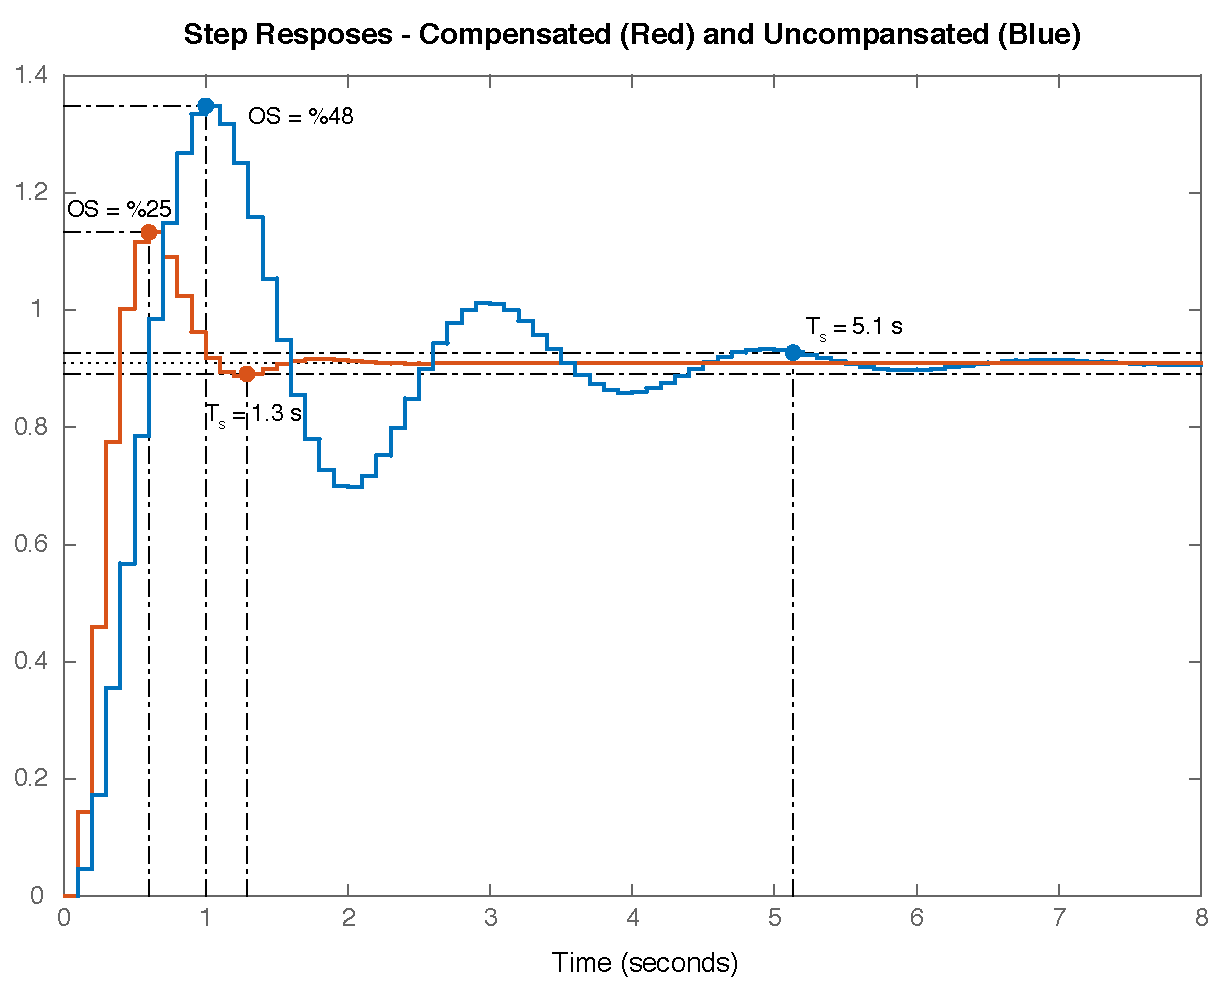
\includegraphics[width=\textwidth]{step}
     \end{center}
 \end{minipage}
     \end{center}
%

% **** This ENDS THE EXAMPLES. DON'T DELETE THE FOLLOWING LINE:
\end{document}